%%%%%%%%%%%%%%%%%%%%%%%%%%%%%%%%%%%%%%%%%%%%%%%%%%%%%%%%%%%%%%%%%%%%%%%%%%%%%%%%%%
% Geometric deep learning for the graph-based midcurve: background and method.
% Numbers come from src/proposal/07_GDL_RESEARCH_REPORT.md. Trained results are in midcurve_gdl_results.tex.
%%%%%%%%%%%%%%%%%%%%%%%%%%%%%%%%%%%%%%%%%%%%%%%%%%%%%%%%%%%%%%%%%%%%%%%%%%%%%%%%%%
\begin{frame}[fragile]\frametitle{}
\begin{center}
{\Large Geometric Deep Learning for the Midcurve}

\vspace{4pt}
EquiCollapse: learning a collapse of the polygon's interior
\end{center}
\end{frame}

%%%%%%%%%%%%%%%%%%%%%%%%%%%%%%%%%%%%%%%%%%%%%%%%%%%%%%%%%%%%%%%%%%%%%%%%%%%%%%%%%%
\begin{frame}[fragile]\frametitle{Geometric Deep Learning in One Slide}
\begin{itemize}
\item Bronstein, Bruna, Cohen and Veli\v{c}kovi\'{c} (2021) describe architectures by the same parts:
  \begin{itemize}
  \item a \textbf{domain} (grid, graph, manifold)
  \item a \textbf{symmetry group} acting on it
  \item \textbf{equivariant layers}, local \textbf{coarsening}, and an invariant readout
  \end{itemize}
\item So the design questions become: what is the right domain, and which symmetries does the task really have?
\end{itemize}

\vspace{4pt}
\begin{center}
\small
\begin{tabular}{@{}ll@{}}
\toprule
\textbf{GDL domain} & \textbf{Midcurve use} \\
\midrule
Grids & Image-based encoder-decoders \\
Graphs & Ring graph, attention over vertices \\
Groups & Rotation and reflection on coordinates \\
Geodesics & Distance through the interior, across opposite walls \\
Gauges & Local wall frames, boundary orientation \\
\bottomrule
\end{tabular}
\end{center}
\end{frame}

%%%%%%%%%%%%%%%%%%%%%%%%%%%%%%%%%%%%%%%%%%%%%%%%%%%%%%%%%%%%%%%%%%%%%%%%%%%%%%%%%%
\begin{frame}[fragile]\frametitle{Which Symmetries Does the Midcurve Have?}
\begin{center}
\small
\begin{tabular}{@{}lc@{}}
\toprule
\textbf{Change to the polygon} & \textbf{Midcurve follows?} \\
\midrule
Different start vertex or listing direction & Yes \\
Translation, rotation, reflection: $E(2)$ & Yes \\
Uniform scaling & Yes \\
Inserting a vertex on a straight wall & Yes \\
Relabelling output nodes & Yes \\
Stretching in one direction (affine) & \textbf{No} \\
\bottomrule
\end{tabular}
\end{center}

\begin{itemize}
\item The medial axis is not affine-equivariant, so that symmetry must not be built in.
\item The right domain is the polygon's \textbf{interior}: the informative neighbour of a wall is the opposite wall, far away along the boundary.
\end{itemize}
\end{frame}

%%%%%%%%%%%%%%%%%%%%%%%%%%%%%%%%%%%%%%%%%%%%%%%%%%%%%%%%%%%%%%%%%%%%%%%%%%%%%%%%%%
\begin{frame}[fragile]\frametitle{Starting Point: the Set Transformer}
\begin{itemize}
\item 12 query slots, an existence flag and Hungarian matching predict the node set; edges come from an inside-polygon minimum spanning tree.
\item Given true nodes, that tree recovers every true edge on these hole-free shapes. \textbf{Edges are not the bottleneck here}.
\item It has no built-in rotation symmetry, and was trained with 90-degree turns only:
\end{itemize}

\begin{center}
\small
\begin{tabular}{@{}lccc@{}}
\toprule
\textbf{Test rotation} & 0$^\circ$ & 5$^\circ$ & 15$^\circ$ \\
\midrule
Correct graph within $0.25w$ & 0.873 & 0.363 & 0.007 \\
\bottomrule
\end{tabular}
\end{center}

{\footnotesize 300 synthetic test shapes, published labels. Expected given the training; continuous rotation augmentation is the fair baseline.}
\end{frame}

%%%%%%%%%%%%%%%%%%%%%%%%%%%%%%%%%%%%%%%%%%%%%%%%%%%%%%%%%%%%%%%%%%%%%%%%%%%%%%%%%%
\begin{frame}[fragile]\frametitle{A Bug Found Along the Way}
\begin{itemize}
\item About 10\% of generated samples have a spurious ground-truth node in the middle of a straight arm.
\item Its position cannot be inferred from the profile, so no model can predict it.
\item Cause: collinear merging compares raw lattice vectors, so it stops once spacings differ.
\end{itemize}

\begin{center}
\small
\begin{tabular}{@{}lcc@{}}
\toprule
\textbf{Correct graph within $0.25w$, iid test} & \textbf{Published labels} & \textbf{Corrected} \\
\midrule
Set transformer (100 epochs) & 0.893 & 0.920 \\
Classical Voronoi & 0.813 & 0.862 \\
\bottomrule
\end{tabular}
\end{center}

{\footnotesize The generator is fixed now; runs shown here were trained before the fix, with cleaned training labels, and report both label sets. The real shapes are unaffected.}
\end{frame}

%%%%%%%%%%%%%%%%%%%%%%%%%%%%%%%%%%%%%%%%%%%%%%%%%%%%%%%%%%%%%%%%%%%%%%%%%%%%%%%%%%
\begin{frame}[fragile]\frametitle{Why a Plain Equivariant Decoder Fails}
\textbf{Claim.} Suppose each query slot has a learned embedding and its position $f_q(P)$ is $E(2)$-equivariant. If a symmetry $g$ maps $P$ onto itself, then
\[
f_q(P) = f_q(gP) = g\, f_q(P),
\]
so every slot sits at a fixed point of the symmetry group of $P$, whatever the weights.

\begin{itemize}
\item I and Plus: the centre only
\item T: the mirror axis only, so the bar's two ends are unreachable
\item L: the diagonal only
\end{itemize}

\vspace{2pt}
Equivariant outputs keeping the input's symmetry is known in general (Smidt et al.\ 2021, Lawrence et al.\ 2025). Here, \textbf{every real benchmark shape is in the failure set}.
\end{frame}

%%%%%%%%%%%%%%%%%%%%%%%%%%%%%%%%%%%%%%%%%%%%%%%%%%%%%%%%%%%%%%%%%%%%%%%%%%%%%%%%%%
\begin{frame}[fragile]\frametitle{Slot Collapse: Numerical Check}
One small network overfitted to one shape; largest distance from a true node to its matched slot, in half-extent units (wall width is about 0.2 to 0.33):

\begin{center}
\small
\begin{tabular}{@{}lccc@{}}
\toprule
\textbf{Shape} & \textbf{Learned slots} & \textbf{Slots ended up} & \textbf{Wall-anchored slots} \\
\midrule
I & 1.000 & at the centre & 0.003 \\
L & 1.382 & on the diagonal & 0.038 \\
T & 1.000 & on the mirror axis & 0.002 \\
Plus & 1.000 & at the centre & 0.006 \\
\bottomrule
\end{tabular}
\end{center}

\textbf{Remedy:} index outputs by input elements. A symmetry then permutes the slots rather than pinning them.
\end{frame}

%%%%%%%%%%%%%%%%%%%%%%%%%%%%%%%%%%%%%%%%%%%%%%%%%%%%%%%%%%%%%%%%%%%%%%%%%%%%%%%%%%
\begin{frame}[fragile]\frametitle{The Idea: Collapse the Interior}
\begin{center}
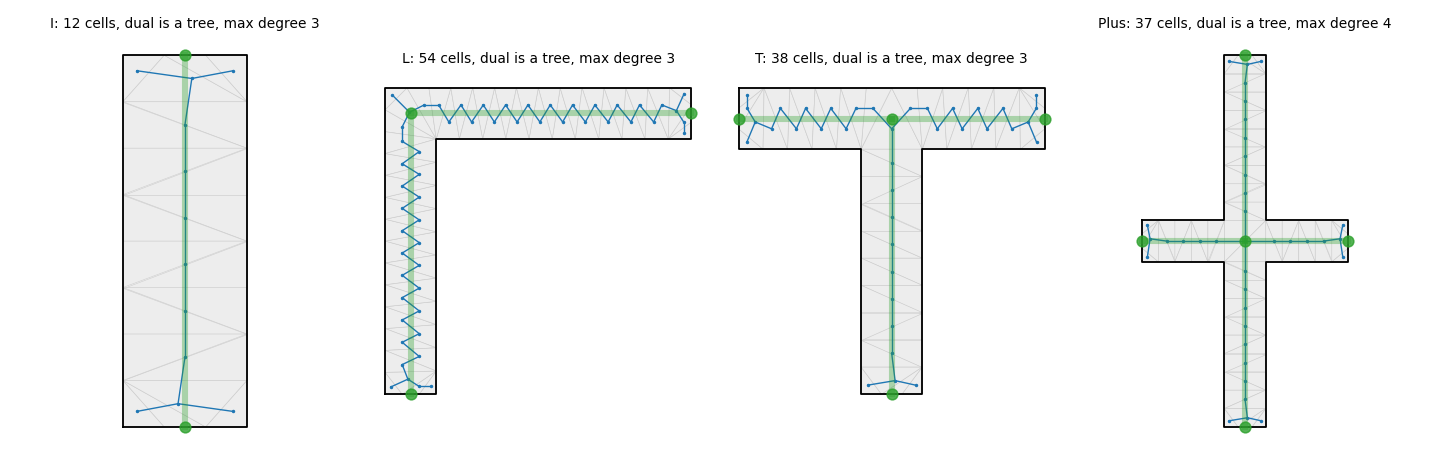
\includegraphics[width=\linewidth,keepaspectratio]{gdl_dual_complex}
\end{center}

{\footnotesize Grey: interior Delaunay cells. Blue: their dual graph. Green: true midcurve.}

\begin{itemize}
\item With all samples on the boundary of a simple polygon, the dual graph is a tree.
\item The midcurve looks like this tree with spurs removed and long chains contracted.
\item So do not \emph{generate} a graph: \textbf{learn which cells to keep} and contract the rest.
\end{itemize}
\end{frame}

%%%%%%%%%%%%%%%%%%%%%%%%%%%%%%%%%%%%%%%%%%%%%%%%%%%%%%%%%%%%%%%%%%%%%%%%%%%%%%%%%%
\begin{frame}[fragile]\frametitle{EquiCollapse: the Pipeline}
\begin{enumerate}
\item \textbf{Canonicalise:} remove collinear vertices; estimate width $\hat{w} = 2A/P$.
\item \textbf{Build the complex:} sample walls at step $0.5\hat{w}$, Delaunay-triangulate, keep interior triangles, merge cocircular neighbours.
\item \textbf{Encode:} message passing on the dual graph with scalar and vector channels, using relative positions only.
\item \textbf{Predict per cell:} a key probability (invariant) and a position offset (equivariant).
\item \textbf{Decode, no learning:}
  \begin{itemize}
  \item contract connected key cells into one output node
  \item repeatedly remove non-key leaves (spurs)
  \item remove non-key degree-2 cells
  \end{itemize}
\end{enumerate}

\vspace{2pt}
Loss: cell-wise BCE plus a robust offset loss. No matching, since cells give the correspondence.
\end{frame}

%%%%%%%%%%%%%%%%%%%%%%%%%%%%%%%%%%%%%%%%%%%%%%%%%%%%%%%%%%%%%%%%%%%%%%%%%%%%%%%%%%
\begin{frame}[fragile]\frametitle{What Holds by Construction, and What Does Not}
\begin{columns}[t]
  \begin{column}[T]{0.5\linewidth}
  \begin{block}{\textcolor{white}{By construction}}
    \begin{itemize}
    \item[\tiny$\blacktriangleright$] Node count is not limited by slots
    \item[\tiny$\blacktriangleright$] Output is a tree on hole-free shapes, for any weights (tested with random scores)
    \item[\tiny$\blacktriangleright$] Network is exactly $E(2)$-equivariant
    \item[\tiny$\blacktriangleright$] No slot collapse: outputs are anchored to cells
    \end{itemize}
  \end{block}
  \end{column}
  \begin{column}[T]{0.5\linewidth}
  \begin{alertblock}{\textcolor{white}{Not guaranteed or not tested}}
    \begin{itemize}
    \item[\tiny$\blacktriangleright$] The complex matching the polygon is checked per shape, not guaranteed
    \item[\tiny$\blacktriangleright$] The tree is abstract: drawn edges can still be geometrically wrong
    \item[\tiny$\blacktriangleright$] Holes: argued, but not implemented
    \item[\tiny$\blacktriangleright$] Width estimate on noisy boundaries
    \end{itemize}
  \end{alertblock}
  \end{column}
\end{columns}
\end{frame}

%%%%%%%%%%%%%%%%%%%%%%%%%%%%%%%%%%%%%%%%%%%%%%%%%%%%%%%%%%%%%%%%%%%%%%%%%%%%%%%%%%
\begin{frame}[fragile]\frametitle{Other GDL Options Considered}
\begin{center}
\small
\begin{tabular}{@{}ll@{}}
\toprule
\textbf{Option} & \textbf{Verdict} \\
\midrule
Rotation augmentation (not GDL) & Cheap control; run first \\
EquiCollapse & Built \\
Equivariant decoder with query slots & Fails on symmetric shapes \\
Frame averaging as main method & Discontinuous at symmetric shapes \\
Steerable or tensor-field networks & More machinery than 2D needs \\
Graph diffusion & Models a distribution; this is a function \\
Autoregressive generation & Ordering is ambiguous on symmetric shapes \\
Cell networks, link prediction & Later, for holes \\
\bottomrule
\end{tabular}
\end{center}
\end{frame}

%%%%%%%%%%%%%%%%%%%%%%%%%%%%%%%%%%%%%%%%%%%%%%%%%%%%%%%%%%%%%%%%%%%%%%%%%%%%%%%%%%
\begin{frame}[fragile]\frametitle{Closest Related Work}
\begin{itemize}
\item \textbf{MidSurfNet} (Ye et al.\ 2026): learned face pairing on B-rep graphs for CAD mid-surfaces.
\item \textbf{Mid-curve completion} (Boussuge and Marc 2021): a CNN patches problem regions of a medial axis.
\item \textbf{Point2Skeleton} (Lin et al.\ 2021): unsupervised skeletal meshes from point clouds.
\item \textbf{ConvPSNet} (Antony et al.\ 2025): learned skeleton of noisy 2D shapes; only a summary has been read so far.
\item \textbf{EMPSN, CW Networks} (2021--2023): equivariant and cell-complex layers, on fixed-output tasks.
\item \textbf{Chordal Axis Transform} (Prasad 1997): a rule-based skeleton on the same kind of structure.
\end{itemize}

\vspace{2pt}
{\footnotesize Our searches found no prior work combining $E(2)$ equivariance, polygon input and learned contraction of the interior complex. They were not a systematic review, so this is not yet a novelty claim.}
\end{frame}
